
\begin{figure}[H]
  {
    \setlength{\tabcolsep}{3.0pt}
    \setlength\cmidrulewidth{\heavyrulewidth} % Make cmidrule = 
    \begin{adjustbox}{width=3cm,center}
      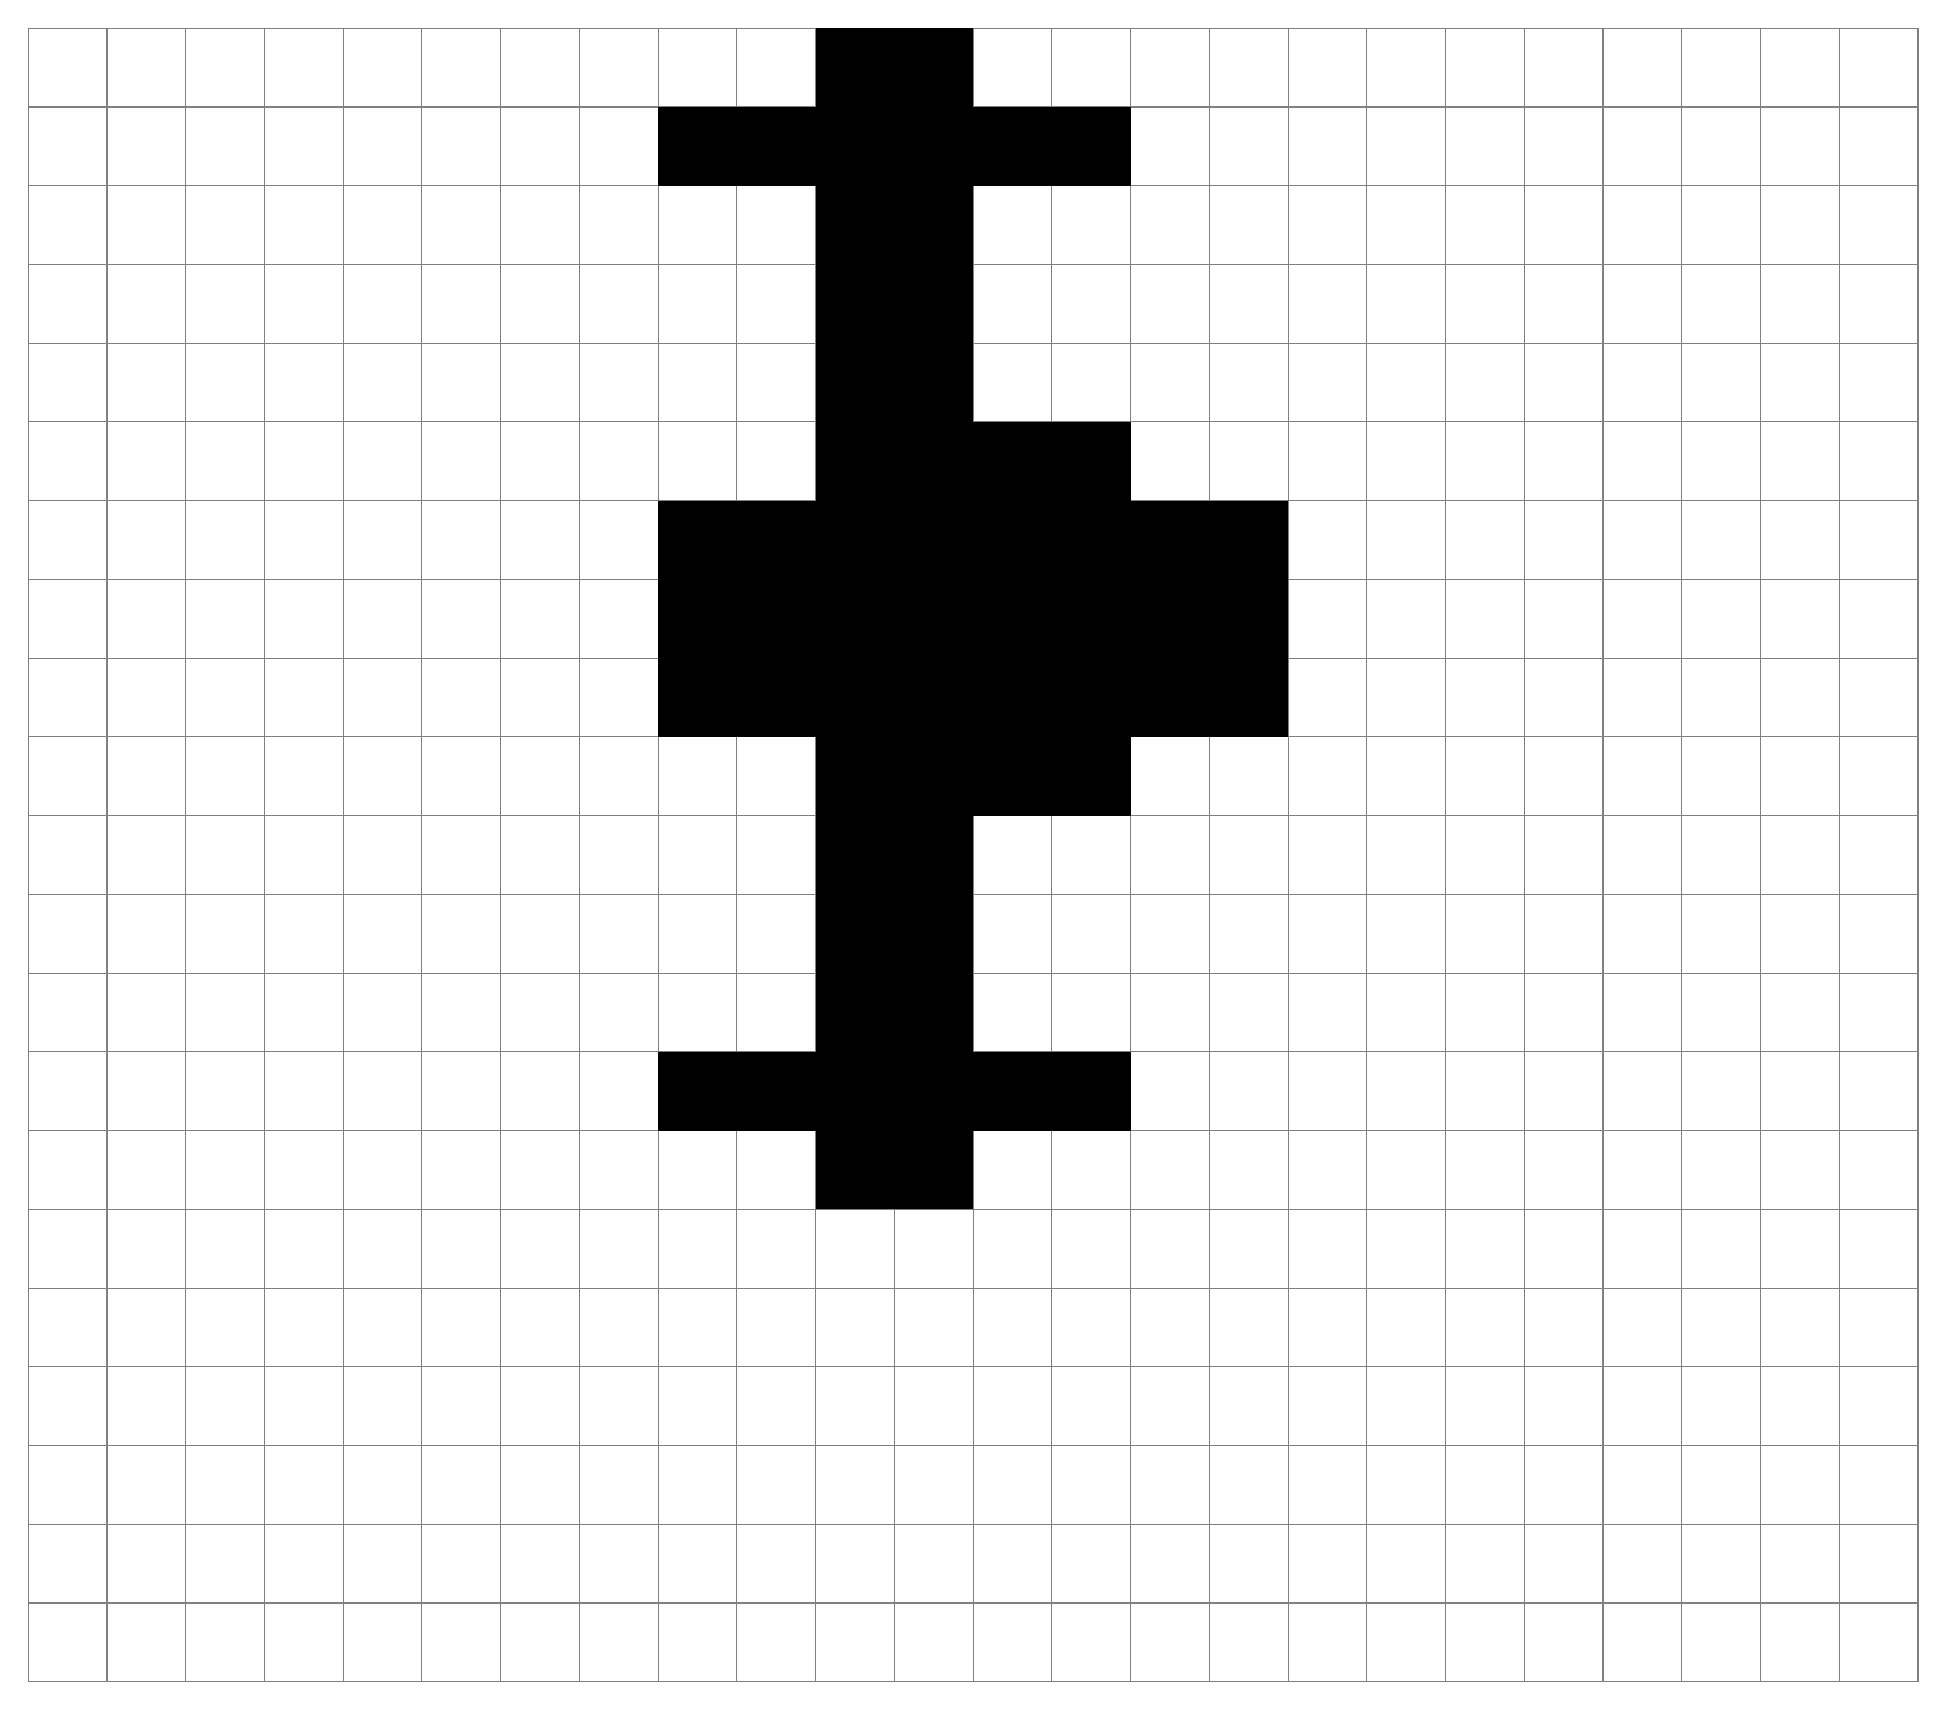
\begin{tikzpicture}

	\draw[step=1.0,gray,thin] (0,0) grid (24,21);
	\fill[\SPRITECOLOR] (10,20) rectangle ++ (1,1);
	\fill[\SPRITECOLOR] (11,20) rectangle ++ (1,1);
	\fill[\SPRITECOLOR] (8,19) rectangle ++ (1,1);
	\fill[\SPRITECOLOR] (9,19) rectangle ++ (1,1);
	\fill[\SPRITECOLOR] (10,19) rectangle ++ (1,1);
	\fill[\SPRITECOLOR] (11,19) rectangle ++ (1,1);
	\fill[\SPRITECOLOR] (12,19) rectangle ++ (1,1);
	\fill[\SPRITECOLOR] (13,19) rectangle ++ (1,1);
	\fill[\MULTICOLORONE] (10,18) rectangle ++ (1,1);
	\fill[\MULTICOLORONE] (11,18) rectangle ++ (1,1);
	\fill[\MULTICOLORONE] (10,17) rectangle ++ (1,1);
	\fill[\MULTICOLORONE] (11,17) rectangle ++ (1,1);
	\fill[\MULTICOLORONE] (10,16) rectangle ++ (1,1);
	\fill[\MULTICOLORONE] (11,16) rectangle ++ (1,1);
	\fill[\MULTICOLORTWO] (10,15) rectangle ++ (1,1);
	\fill[\MULTICOLORTWO] (11,15) rectangle ++ (1,1);
	\fill[\SPRITECOLOR] (12,15) rectangle ++ (1,1);
	\fill[\SPRITECOLOR] (13,15) rectangle ++ (1,1);
	\fill[\MULTICOLORTWO] (8,14) rectangle ++ (1,1);
	\fill[\MULTICOLORTWO] (9,14) rectangle ++ (1,1);
	\fill[\SPRITECOLOR] (10,14) rectangle ++ (1,1);
	\fill[\SPRITECOLOR] (11,14) rectangle ++ (1,1);
	\fill[\SPRITECOLOR] (12,14) rectangle ++ (1,1);
	\fill[\SPRITECOLOR] (13,14) rectangle ++ (1,1);
	\fill[\SPRITECOLOR] (14,14) rectangle ++ (1,1);
	\fill[\SPRITECOLOR] (15,14) rectangle ++ (1,1);
	\fill[\SPRITECOLOR] (8,13) rectangle ++ (1,1);
	\fill[\SPRITECOLOR] (9,13) rectangle ++ (1,1);
	\fill[\SPRITECOLOR] (10,13) rectangle ++ (1,1);
	\fill[\SPRITECOLOR] (11,13) rectangle ++ (1,1);
	\fill[\SPRITECOLOR] (12,13) rectangle ++ (1,1);
	\fill[\SPRITECOLOR] (13,13) rectangle ++ (1,1);
	\fill[\SPRITECOLOR] (14,13) rectangle ++ (1,1);
	\fill[\SPRITECOLOR] (15,13) rectangle ++ (1,1);
	\fill[\SPRITECOLOR] (8,12) rectangle ++ (1,1);
	\fill[\SPRITECOLOR] (9,12) rectangle ++ (1,1);
	\fill[\SPRITECOLOR] (10,12) rectangle ++ (1,1);
	\fill[\SPRITECOLOR] (11,12) rectangle ++ (1,1);
	\fill[\SPRITECOLOR] (12,12) rectangle ++ (1,1);
	\fill[\SPRITECOLOR] (13,12) rectangle ++ (1,1);
	\fill[\SPRITECOLOR] (14,12) rectangle ++ (1,1);
	\fill[\SPRITECOLOR] (15,12) rectangle ++ (1,1);
	\fill[\SPRITECOLOR] (10,11) rectangle ++ (1,1);
	\fill[\SPRITECOLOR] (11,11) rectangle ++ (1,1);
	\fill[\SPRITECOLOR] (12,11) rectangle ++ (1,1);
	\fill[\SPRITECOLOR] (13,11) rectangle ++ (1,1);
	\fill[\MULTICOLORONE] (10,10) rectangle ++ (1,1);
	\fill[\MULTICOLORONE] (11,10) rectangle ++ (1,1);
	\fill[\MULTICOLORONE] (10,9) rectangle ++ (1,1);
	\fill[\MULTICOLORONE] (11,9) rectangle ++ (1,1);
	\fill[\MULTICOLORONE] (10,8) rectangle ++ (1,1);
	\fill[\MULTICOLORONE] (11,8) rectangle ++ (1,1);
	\fill[\SPRITECOLOR] (8,7) rectangle ++ (1,1);
	\fill[\SPRITECOLOR] (9,7) rectangle ++ (1,1);
	\fill[\SPRITECOLOR] (10,7) rectangle ++ (1,1);
	\fill[\SPRITECOLOR] (11,7) rectangle ++ (1,1);
	\fill[\SPRITECOLOR] (12,7) rectangle ++ (1,1);
	\fill[\SPRITECOLOR] (13,7) rectangle ++ (1,1);
	\fill[\SPRITECOLOR] (10,6) rectangle ++ (1,1);
	\fill[\SPRITECOLOR] (11,6) rectangle ++ (1,1);

      \end{tikzpicture}
    \end{adjustbox}
  }\caption{BOLAS3}
\end{figure}
